% Pharma Research Agent - 10-minute presentation (Beamer, 16:9)
% Build:  pdflatex presentation.tex   (run twice)   - or upload this folder to Overleaf.
\documentclass[aspectratio=169,11pt]{beamer}

\usepackage[T1]{fontenc}
\usepackage[utf8]{inputenc}
\usepackage{lmodern}
\usepackage{amsmath}
\usepackage{booktabs}
\usepackage{tabularx}
\usepackage{listings}
\usepackage{tikz}
\usetikzlibrary{arrows.meta,positioning,fit,calc}

% ---------- Look and feel ----------
\definecolor{navy}{HTML}{1E3A8A}
\definecolor{accent}{HTML}{2563EB}
\definecolor{soft}{HTML}{EEF2FF}
\definecolor{okgreen}{HTML}{15803D}
\definecolor{warnorange}{HTML}{B45309}
\definecolor{grey}{HTML}{6B7280}

\usetheme{default}
\setbeamertemplate{navigation symbols}{}
\setbeamercolor{frametitle}{fg=navy}
\setbeamercolor{title}{fg=navy}
\setbeamercolor{structure}{fg=accent}
\setbeamercolor{block title}{bg=accent,fg=white}
\setbeamercolor{block body}{bg=soft}
\setbeamerfont{frametitle}{series=\bfseries,size=\Large}
\setbeamertemplate{itemize items}[circle]
\setbeamertemplate{footline}{%
  \hfill{\color{grey}\scriptsize Pharma Research Agent \quad \insertframenumber/\inserttotalframenumber}\hspace{1em}\vspace{0.6em}}

\lstset{
  language=Python, basicstyle=\ttfamily\scriptsize, keywordstyle=\color{accent}\bfseries,
  commentstyle=\color{grey}\itshape, stringstyle=\color{okgreen}, showstringspaces=false,
  frame=single, rulecolor=\color{soft}, backgroundcolor=\color{soft}, columns=fullflexible,
  breaklines=true
}

\newcommand{\file}[1]{\texttt{\small #1}}
\newcommand{\good}[1]{{\color{okgreen}\textbf{#1}}}
\newcommand{\warn}[1]{{\color{warnorange}\textbf{#1}}}

\title{Pharma Research Agent}
\subtitle{An agentic assistant that answers compound questions\\ about drug labels, with citations and a built-in reviewer}
\author{Your Name}        % <-- edit
\institute{GenAI Bootcamp -- Coding Assignment}
\date{November 2026}

\begin{document}

% =====================================================================
\begin{frame}
  \titlepage
\end{frame}

% =====================================================================
\begin{frame}{The problem}
  \begin{columns}[T]
    \begin{column}{0.55\textwidth}
      \textbf{Goal:} answer \emph{compound} pharmacology questions from a local corpus of
      21 files (FDA DailyMed labels, MedlinePlus monographs, a glossary).
      \vspace{0.6em}

      \textbf{Required behaviour}
      \begin{enumerate}
        \item \textbf{Plan} -- split the question into sub-questions
        \item \textbf{Retrieve} -- in-memory similarity search
        \item \textbf{Tools} -- at least two, chosen by the agent
        \item \textbf{Review} -- a critic flags unsupported / ambiguous claims
        \item \textbf{Answer} -- cite source files + medical disclaimer
      \end{enumerate}
    \end{column}
    \begin{column}{0.42\textwidth}
      \begin{block}{Example questions}
        \small
        \begin{itemize}
          \item Main contraindications of warfarin?
          \item Compare warfarin and apixaban contraindications.
          \item Warfarin + sertraline: bleeding risk and monitoring?
          \item eGFR 25 mL/min: is metformin contraindicated?
        \end{itemize}
      \end{block}
      \vspace{0.3em}
      {\small Delivered as a Docker container: \texttt{GET /health}, \texttt{POST /ask}, web UI.}
    \end{column}
  \end{columns}
\end{frame}

% =====================================================================
\begin{frame}{The result: a chat that shows its work}
  \begin{columns}[c]
    \begin{column}{0.58\textwidth}
      \centering
      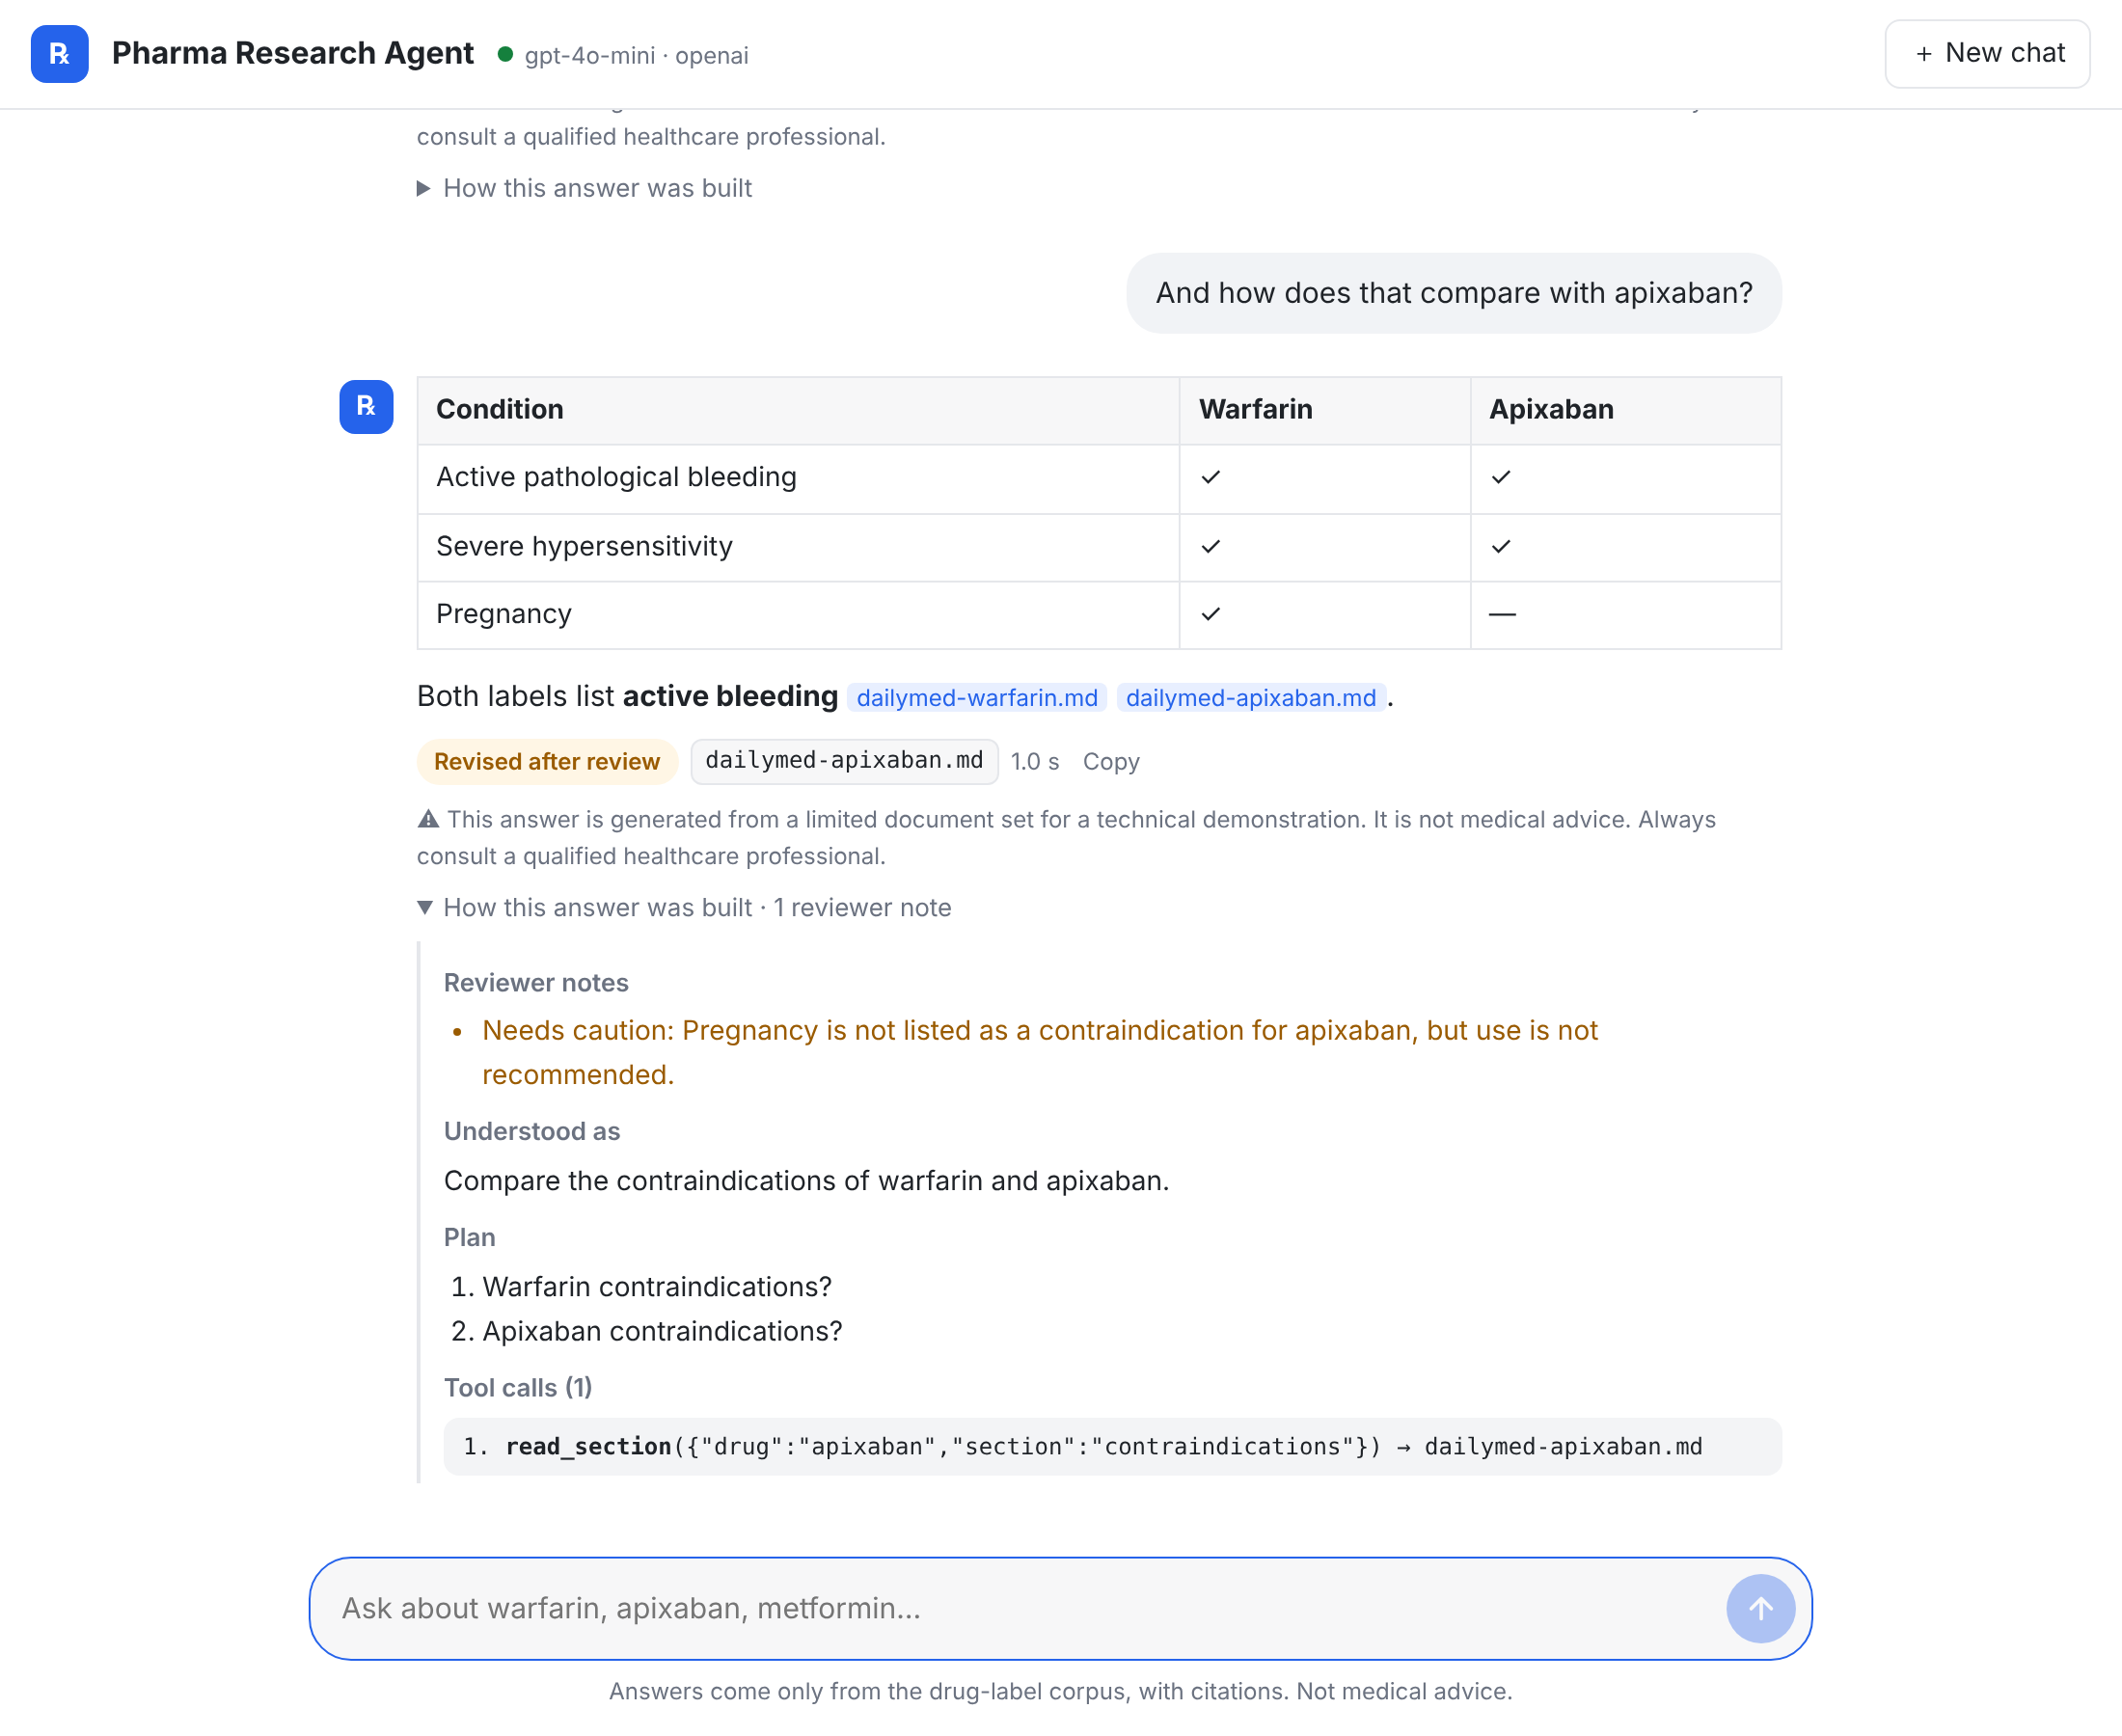
\includegraphics[width=\textwidth]{figures/ui-chat.png}
    \end{column}
    \begin{column}{0.4\textwidth}
      \small
      \begin{itemize}
        \item Answer in Markdown with \textbf{inline citations} \file{[dailymed-warfarin.md]}
        \item \good{Verified by reviewer} or \warn{Revised after review} badge
        \item Reviewer notes, the \textbf{plan} and the full \textbf{tool trace}
        \item Follow-up questions in the same chat (\emph{``and for apixaban?''})
        \item Disclaimer always present, added by code
      \end{itemize}
    \end{column}
  \end{columns}
\end{frame}

% =====================================================================
\begin{frame}{Tools and technology choices}
  \footnotesize
  \renewcommand{\arraystretch}{1.12}
  \begin{tabularx}{\textwidth}{@{}l l X@{}}
    \toprule
    \textbf{Need} & \textbf{Choice} & \textbf{Why} \\
    \midrule
    LLM access & OpenAI Python SDK & Works with OpenAI, the LiteLLM proxy and Groq via one client \\
    Orchestration & \textbf{own loop} ($\sim$40 lines) & Every step readable, debuggable and returned as a trace; no hidden prompts \\
    Tool use & native function calling & The LLM picks the tool -- nothing hard-coded \\
    Vector search & NumPy matrix & 572 chunks fit in memory; no vector DB to run \\
    Embeddings & API embeddings / local TF-IDF & Groq has no embeddings API $\rightarrow$ own TF-IDF \\
    API & FastAPI + Pydantic & Validated input/output, typed JSON responses \\
    UI & one HTML file, plain JS & No build step; served by the API itself \\
    Delivery & Docker (\texttt{python:3.12-slim}) & Self-contained; graders inject their own \texttt{.env} \\
    \bottomrule
  \end{tabularx}
  \vspace{0.5em}

  {\color{grey}\footnotesize $\approx$ 860 lines of Python, one file per concern: \file{corpus.py}, \file{tools.py}, \file{agent.py}, \file{prompts.py}, \file{llm.py}, \file{main.py}.}
\end{frame}

% =====================================================================
\begin{frame}{Architecture and workflow}
  \centering
  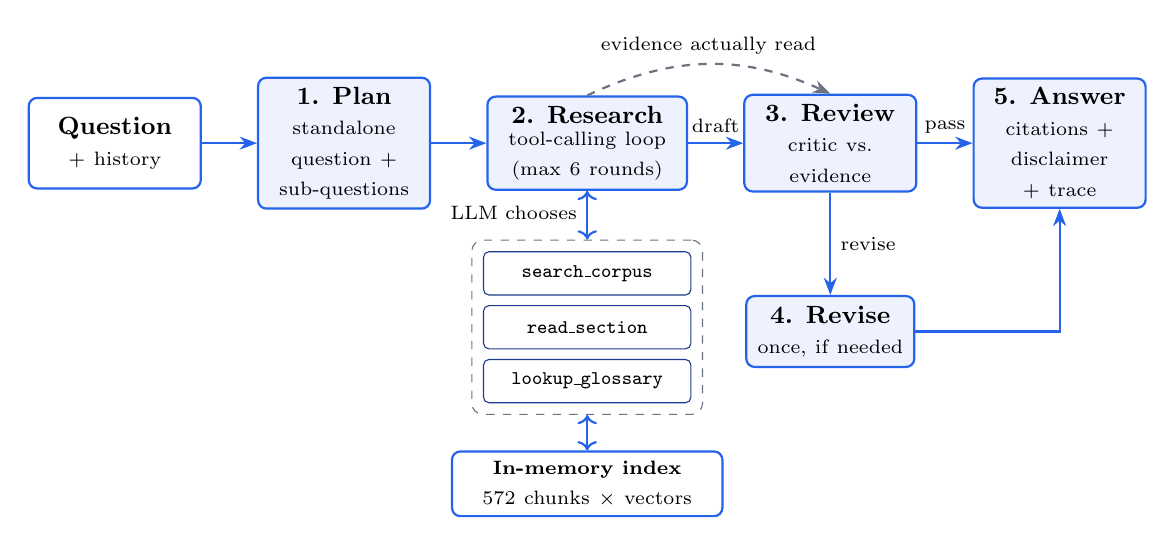
\begin{tikzpicture}[
      node distance=0.55cm and 0.7cm,
      box/.style={draw=accent, fill=soft, rounded corners=3pt, thick, align=center,
                   minimum height=1.15cm, text width=1.95cm, font=\small},
      tool/.style={draw=navy, fill=white, rounded corners=2pt, align=center, font=\scriptsize\ttfamily,
                   minimum height=0.55cm, text width=2.4cm},
      arr/.style={-{Stealth[length=2.2mm]}, thick, accent}]
    \node[box, fill=white] (q) {\textbf{Question}\\ \scriptsize + history};
    \node[box, right=of q] (plan) {\textbf{1. Plan}\\ \scriptsize standalone question + sub-questions};
    \node[box, right=of plan, text width=2.3cm] (research) {\textbf{2. Research}\\ \scriptsize tool-calling loop\\ (max 6 rounds)};
    \node[box, right=of research] (review) {\textbf{3. Review}\\ \scriptsize critic vs.\ evidence};
    \node[box, right=of review] (answer) {\textbf{5. Answer}\\ \scriptsize citations + disclaimer + trace};

    \node[box, below=1.3cm of review, text width=1.9cm, minimum height=0.9cm] (revise) {\textbf{4. Revise}\\ \scriptsize once, if needed};

    \node[tool, below=1.45cm of research] (t2) {read\_section};
    \node[tool, above=0.12cm of t2] (t1) {search\_corpus};
    \node[tool, below=0.12cm of t2] (t3) {lookup\_glossary};
    \node[draw=grey, dashed, rounded corners, fit=(t1)(t2)(t3), inner sep=4pt] (tools) {};
    \node[box, below=0.45cm of tools, text width=3.2cm, minimum height=0.8cm, fill=white] (index)
         {\scriptsize \textbf{In-memory index}\\ 572 chunks $\times$ vectors};

    \draw[arr] (q) -- (plan);
    \draw[arr] (plan) -- (research);
    \draw[arr] (research) -- node[above, font=\scriptsize, black]{draft} (review);
    \draw[arr] (review) -- node[above, font=\scriptsize, black]{pass} (answer);
    \draw[arr] (review) -- node[right, font=\scriptsize, black]{revise} (revise);
    \draw[arr] (revise) -| (answer);
    \draw[arr, <->] (research) -- node[left, font=\scriptsize, black, pos=0.45]{LLM chooses} (tools);
    \draw[arr, <->] (tools) -- (index);
    \draw[arr, dashed, grey] (research.north) to[bend left=25] node[above, font=\scriptsize, black]{evidence actually read} (review.north);
  \end{tikzpicture}

  \vspace{0.3em}
  {\small LLM calls per question: \textbf{3 minimum} (plan, research, review), \textbf{about 10 maximum}.}
\end{frame}

% =====================================================================
\begin{frame}[fragile]{Step 1 -- Planning (and follow-up questions)}
  \begin{columns}[T]
    \begin{column}{0.5\textwidth}
      \begin{itemize}
        \item One LLM call in \textbf{JSON mode}
        \item Output: 1--4 self-contained sub-questions + drugs involved
        \item Plan is injected into the researcher's system prompt
        \item Robust parsing: falls back to the original question if the JSON is unusable
      \end{itemize}
      \vspace{0.5em}
      \textbf{Conversation for free:} the planner also rewrites a follow-up into a
      \emph{standalone question}. The rest of the pipeline never sees the history
      $\Rightarrow$ no extra LLM call.
    \end{column}
    \begin{column}{0.47\textwidth}
\begin{lstlisting}[language={}]
History: "Contraindications of warfarin?"
New:     "And for apixaban?"

{ "standalone_question":
    "What are the contraindications
     of apixaban?",
  "sub_questions": [
    "What are apixaban's
     contraindications?"],
  "drugs": ["apixaban"] }
\end{lstlisting}
    \end{column}
  \end{columns}
\end{frame}

% =====================================================================
\begin{frame}{Algorithm 1 -- Section-aware chunking}
  \begin{columns}[T]
    \begin{column}{0.52\textwidth}
      \textbf{Idea:} drug labels are organised by sections, so chunk along the
      Markdown heading tree instead of fixed-size windows.
      \begin{enumerate}
        \item Walk the lines; keep the stack of headings (H1--H6)
        \item One chunk per (sub)section, labelled with its path:\\
              \file{7 DRUG INTERACTIONS > 7.3 Drugs that Increase Bleeding Risk}
        \item Sections longer than 1\,500 chars are split on paragraph boundaries
        \item Each chunk is embedded \emph{with} its header \file{[file] title > section}
      \end{enumerate}
    \end{column}
    \begin{column}{0.45\textwidth}
      \begin{block}{Why}
        \small
        \begin{itemize}
          \item Every hit maps to a citable \textbf{file + section}
          \item Passages stay self-contained (no list cut in half)
          \item The header puts the \textbf{drug name} into the vector, so ``contraindications'' of warfarin and apixaban don't look identical
        \end{itemize}
      \end{block}
      \vspace{0.3em}
      {\small 21 files $\rightarrow$ \textbf{572 chunks}, median $\approx$ 590 characters.}
    \end{column}
  \end{columns}
\end{frame}

% =====================================================================
\begin{frame}{Algorithm 2 -- In-memory similarity search}
  \begin{columns}[T]
    \begin{column}{0.5\textwidth}
      All chunk vectors are L2-normalised once and stacked in a matrix
      $V \in \mathbb{R}^{n\times d}$. For a query vector $q$:
      \[
        \text{score} = V\,\hat q, \qquad \hat q = \frac{q}{\lVert q\rVert}
      \]
      i.e.\ \textbf{cosine similarity} with one matrix-vector product, then top-$k$ ($k=5$).
      \vspace{0.4em}

      \textbf{Drug filter:} \texttt{search\_corpus(query, drug)} restricts candidates to that drug's files.
    \end{column}
    \begin{column}{0.47\textwidth}
      \begin{block}{Why the filter matters}
        \small
        In ``warfarin + sertraline'', warfarin's long bleeding sections dominate the ranking.
        Searching each drug separately guarantees both labels are read.
      \end{block}
      \vspace{0.4em}
      \begin{block}{Startup}
        \small
        The index is built in a \textbf{background thread} when the API starts,
        so \texttt{/health} answers 200 immediately.
      \end{block}
    \end{column}
  \end{columns}
\end{frame}

% =====================================================================
\begin{frame}{Algorithm 3 -- Local TF-IDF embeddings (no embeddings API)}
  \begin{columns}[T]
    \begin{column}{0.55\textwidth}
      Groq has no embeddings endpoint, so I wrote a TF-IDF vectoriser in NumPy:
      \begin{itemize}
        \item Tokens: lower-cased words minus stop words, \textbf{plus bigrams} (\texttt{renal\_impairment})
        \item Sub-linear term frequency and smoothed IDF:
        \[
          w_{t,c} = \bigl(1+\log \mathrm{tf}_{t,c}\bigr)\cdot\Bigl(\log\frac{1+N}{1+\mathrm{df}_t}+1\Bigr)
        \]
        \item L2-normalised $\Rightarrow$ the \emph{same} cosine search as with API embeddings
      \end{itemize}
      {\small Vocabulary learnt from the corpus: \textbf{31\,457 terms}.}
    \end{column}
    \begin{column}{0.42\textwidth}
      \begin{block}{Why it works here}
        \small
        Drug-label questions hinge on \textbf{exact terms}: drug names, section names,
        ``eGFR'', ``INR''. Lexical matching is strong on this vocabulary.
      \end{block}
      \vspace{0.3em}
      \begin{block}{Trade-off}
        \small
        No synonyms (``bleeding'' $\neq$ ``hemorrhage''). Semantic API embeddings are used
        whenever available (default with OpenAI / LiteLLM).
      \end{block}
    \end{column}
  \end{columns}
\end{frame}

% =====================================================================
\begin{frame}[fragile]{Step 2 -- Agent-driven tool use}
  \begin{columns}[T]
    \begin{column}{0.37\textwidth}
      \small
      \textbf{Three local tools}\\[0.3em]
      {\footnotesize
      \texttt{search\_corpus} -- open questions\\
      \texttt{read\_section} -- \emph{complete} lists\\
      \texttt{lookup\_glossary} -- INR, eGFR\dots\par}
      \vspace{0.6em}
      \begin{itemize}
        \item Schemas sent as JSON:\\ \textbf{the model decides}
        \item Unknown section $\Rightarrow$ the tool lists the available ones and the agent retries
        \item Max 6 rounds, then a forced answer
      \end{itemize}
    \end{column}
    \begin{column}{0.6\textwidth}
\begin{lstlisting}[basicstyle=\ttfamily\fontsize{7.5}{9.2}\selectfont]
for _ in range(MAX_TOOL_ROUNDS):
    msg = llm.chat(messages, tools=TOOL_SPECS)
    if not msg.tool_calls:        # the model is done
        return msg.content, evidence, steps
    messages.append(assistant_msg(msg))
    for call in msg.tool_calls:
        name = call.function.name
        args = parse_json(call.function.arguments)
        output, chunks = run_tool(index, name, args)
        evidence.extend(chunks)   # for the critic
        steps.append(ToolStep(tool=name, ...))  # UI trace
        messages.append({"role": "tool",
                         "tool_call_id": call.id,
                         "content": output})

# budget exhausted: answer with what was read
msg = llm.chat(messages, tools=TOOL_SPECS,
               tool_choice="none")
\end{lstlisting}
    \end{column}
  \end{columns}
\end{frame}

% =====================================================================
\begin{frame}{Steps 3--4 -- Critic and revision}
  \begin{columns}[T]
    \begin{column}{0.5\textwidth}
      \small
      \textbf{Critic} = a second LLM call with a strict reviewer prompt. It receives:
      \begin{itemize}
        \item the question and the draft answer
        \item \textbf{exactly the passages the agent read} (deduplicated, capped at 40k chars)
      \end{itemize}
      It returns JSON:
      \begin{itemize}
        \item \texttt{unsupported\_claims} -- not in the evidence
        \item \texttt{ambiguous\_claims} -- clinically risky without nuance
        \item \texttt{missing} -- parts of the question not answered
        \item \texttt{verdict}: \good{pass} / \warn{revise} + feedback
      \end{itemize}
    \end{column}
    \begin{column}{0.47\textwidth}
      \begin{block}{Why give it the evidence?}
        \small
        Without it, the critic can only judge plausibility. With it, it can catch claims
        that came from the model's own memory instead of the corpus.
      \end{block}
      \vspace{0.4em}
      \begin{block}{Revision}
        \small
        If \warn{revise}: \textbf{one} rewrite using the feedback and the same evidence.
        Bounded cost and latency; the notes are shown to the user either way.
      \end{block}
    \end{column}
  \end{columns}
\end{frame}

% =====================================================================
\begin{frame}{Step 5 -- Safety by construction, not by prompt}
  \begin{itemize}
    \item \textbf{Disclaimer added by code} (\file{config.DISCLAIMER}) -- the model cannot forget it
    \item \textbf{Sources = cited $\cap$ read}: file names are extracted from the answer and kept
          only if a tool actually returned that file $\Rightarrow$ an invented citation never reaches the user
    \item \textbf{Answer only from the corpus}: prompts forbid outside knowledge; the critic enforces it
    \item \textbf{Bounded agent}: max 6 tool rounds, 1 revision, evidence cap, SDK retries on rate limits
    \item \textbf{Full transparency}: plan, every tool call and its sources, reviewer verdict and notes,
          latency -- all returned by \texttt{POST /ask} and shown in the UI
  \end{itemize}
  \vspace{0.5em}
  \begin{block}{Response of \texttt{POST /ask}}
    \small\ttfamily
    question, standalone\_question, answer, sources[], plan[], steps[\{tool, arguments, sources\}],
    review\{verdict, unsupported\_claims, ambiguous\_claims, missing, revised\}, disclaimer, latency\_ms
  \end{block}
\end{frame}

% =====================================================================
\begin{frame}{Testing and evaluation}
  \begin{columns}[T]
    \begin{column}{0.48\textwidth}
      \small
      \textbf{15 offline unit tests} (\texttt{pytest}, no network, < 1 s)
      \begin{itemize}
        \item Fake hashed bag-of-words embedding
        \item \textbf{Scripted fake LLM} that returns tool calls, so the whole loop and the API run end to end
        \item Chunking, tools, TF-IDF ranking, follow-up rewriting, input validation
      \end{itemize}
      \vspace{0.3em}
      \textbf{Evaluation script} \texttt{python -m app.evaluate}
      \begin{itemize}
        \item Runs the 4 public questions in-process or against the container (\texttt{-{}-url})
        \item Pass = every expected source file is cited
      \end{itemize}
    \end{column}
    \begin{column}{0.49\textwidth}
      \small
      \renewcommand{\arraystretch}{1.2}
      \begin{tabularx}{\textwidth}{@{}X c c@{}}
        \toprule
        \textbf{Question} & \textbf{Sources} & \textbf{Review} \\
        \midrule
        Warfarin contra\-indications & ?/1 & ? \\
        Warfarin vs apixaban & ?/2 & ? \\
        Warfarin + sertraline & ?/2 & ? \\
        Metformin, eGFR 25 & ?/1 & ? \\
        \bottomrule
      \end{tabularx}
      \vspace{0.3em}

      {\color{warnorange}\footnotesize Fill in with the output of \texttt{python -m app.evaluate} on the provided key.}
    \end{column}
  \end{columns}
\end{frame}

% =====================================================================
\begin{frame}{Challenges and how I solved them}
  \footnotesize
  \renewcommand{\arraystretch}{1.18}
  \begin{tabularx}{\textwidth}{@{}>{\raggedright\arraybackslash}p{0.36\textwidth} X@{}}
    \toprule
    \textbf{Challenge} & \textbf{Solution} \\
    \midrule
    Similarity search misses items of long lists (``list \emph{all} contraindications'') & \texttt{read\_section} tool returns the whole section; the agent chooses it \\
    In multi-drug questions one drug crowds out the other & \texttt{drug} filter on \texttt{search\_corpus}; prompt: check each drug in its own files \\
    Groq has no embeddings API & Own TF-IDF vectoriser with bigrams, same cosine search \\
    Model may cite files it never read & \texttt{sources} = cited $\cap$ actually read \\
    LLM JSON is not always clean & JSON mode + tolerant parser + safe fallbacks \\
    Rate limits on free tiers & SDK retries with back-off; configurable evidence cap \\
    Slow startup (embedding the corpus) & Index built in a background thread; \texttt{/health} is instant \\
    Follow-up questions (``and for apixaban?'') & Planner rewrites them into standalone questions \\
    Testing an LLM app reliably & Scripted fake LLM + fake embeddings, fully offline \\
    \bottomrule
  \end{tabularx}
\end{frame}

% =====================================================================
\begin{frame}{Limits of the current solution}
  \begin{columns}[T]
    \begin{column}{0.5\textwidth}
      \textbf{Quality}
      \begin{itemize}
        \item Critic is the \textbf{same LLM} -- it can share the writer's blind spots
        \item Only \textbf{one revision}, and the revised answer is not re-reviewed
        \item Citations checked at \textbf{file level}, not claim by claim
        \item TF-IDF has no synonyms; brand names (Coumadin, Eliquis) are not mapped to files
        \item Evaluation only checks sources, not answer correctness
      \end{itemize}
    \end{column}
    \begin{column}{0.47\textwidth}
      \textbf{Engineering}
      \begin{itemize}
        \item \textbf{Latency}: 3--10 sequential LLM calls, no streaming; UI progress labels are timed, not real events
        \item Index rebuilt (re-embedded) at every start; nothing cached on disk
        \item In-memory index fits $\sim$20 files, not a large label database
        \item No authentication or rate limiting; chat history kept only in the browser
      \end{itemize}
    \end{column}
  \end{columns}
\end{frame}

% =====================================================================
\begin{frame}{What I would improve next}
  \begin{columns}[T]
    \begin{column}{0.5\textwidth}
      \textbf{Answer quality}
      \begin{itemize}
        \item \textbf{Hybrid retrieval}: BM25 + embeddings fused with reciprocal rank fusion, then a cross-encoder re-ranker
        \item \textbf{Claim-level grounding}: split the answer into claims, verify each against its cited passage
        \item Critic on a different / stronger model; loop until pass (with a budget)
        \item Drug synonym and brand-name map
      \end{itemize}
    \end{column}
    \begin{column}{0.47\textwidth}
      \textbf{Product and operations}
      \begin{itemize}
        \item \textbf{Streaming} (SSE) of real progress and tokens to the UI
        \item Parallel tool calls and async LLM calls to cut latency
        \item Cache embeddings on disk; vector DB if the corpus grows
        \item Larger eval set with an LLM-as-judge on expected facts
        \item Tracing of tokens, cost and latency per step
      \end{itemize}
    \end{column}
  \end{columns}
\end{frame}

% =====================================================================
\begin{frame}{How I worked: AI-assisted development}
  \begin{itemize}
    \item Built with \textbf{Claude} as a coding assistant; its instructions are committed in \file{CLAUDE.md}:
      \begin{itemize}
        \item plain Python, no framework, one file per concern
        \item tool choice by the LLM only; disclaimer added by code
        \item all LLM access through \file{app/llm.py}; dependencies pinned
        \item tests must run offline with fakes
      \end{itemize}
    \item Workflow: change code $\rightarrow$ \texttt{pytest -q} $\rightarrow$ check the API and UI manually
    \item I reviewed every file and can explain each design decision
  \end{itemize}
  \vspace{0.6em}
  \begin{block}{Run it}
    \small\ttfamily
    docker build -t agent . \&\& docker run -p 8000:8000 -{}-env-file .env agent\\
    python -m app.evaluate -{}-url http://localhost:8000
  \end{block}
\end{frame}

% =====================================================================
\begin{frame}{Summary}
  \begin{itemize}
    \item A \textbf{transparent agent}: plan $\rightarrow$ tool-driven research $\rightarrow$ grounded critic $\rightarrow$ cited answer
    \item \textbf{Retrieval designed for drug labels}: section-aware chunks, drug filter, full-section reads, glossary
    \item \textbf{Safety in code}: disclaimer, verified sources, bounded loop
    \item \textbf{Provider-agnostic}: OpenAI / LiteLLM with embeddings, or Groq with local TF-IDF
    \item \textbf{Usable}: chat UI with follow-ups, Docker, offline tests, evaluation script
  \end{itemize}
  \vspace{1.2em}
  \centering
  {\Large\color{navy}\textbf{Thank you -- questions?}}\\[0.6em]
  {\small\color{grey} Live demo: \texttt{http://localhost:8000}}
\end{frame}

\end{document}
